\chapter{Memory Hierarchy and Caches}

Processors are much faster than main memory (a DRAM access takes on the
order of 100 processor cycles). We want memory that is as large as the
cheapest technology and as fast as the fastest. The trick is a
\textbf{memory hierarchy}: small fast memories close to the processor hold
copies of the data most likely to be used next.

\section{Locality}

\begin{definition}
\textbf{Temporal locality}: an item referenced recently is likely to be
referenced again soon (loop variables, instructions in a loop).
\textbf{Spatial locality}: items near a recently referenced item are likely
to be referenced soon (sequential instructions, array traversal).
\end{definition}

\begin{center}
\begin{tabular}{llll}
\toprule
Level & Technology & Typical access time & Typical size \\
\midrule
Registers & flip-flops & $<1$\,ns & $\sim$100s of bytes \\
L1 cache & SRAM & $\sim$1\,ns & 32--64\,KB \\
L2/L3 cache & SRAM & 3--20\,ns & MBs \\
Main memory & DRAM & 50--100\,ns & GBs \\
Disk / SSD & magnetic / flash & $\mu$s--ms & TBs \\
\bottomrule
\end{tabular}
\end{center}

\begin{figure}[H]
\centering
\begin{tikzpicture}[font=\small, >=Stealth]
  \foreach \i/\lab/\c in {0/Registers/red!20, 1/L1 cache/orange!20, 2/{L2/L3 cache}/yellow!25, 3/Main memory (DRAM)/green!15, 4/{Disk / SSD}/blue!12} {
    \pgfmathsetmacro{\wt}{0.6 + 0.75*\i}
    \pgfmathsetmacro{\wb}{0.6 + 0.75*(\i+1)}
    \filldraw[fill=\c, draw=black] (-\wt,-0.8*\i) -- (\wt,-0.8*\i) -- (\wb,-0.8*\i-0.8) -- (-\wb,-0.8*\i-0.8) -- cycle;
    \node at (0,-0.8*\i-0.4) {\lab};
  }
  \draw[->, thick] (-4.8,-4) -- node[left, align=center, font=\scriptsize]{faster,\\smaller,\\costlier\\per byte} (-4.8,0);
  \draw[->, thick] (4.8,0) -- node[right, align=center, font=\scriptsize]{larger,\\slower,\\cheaper} (4.8,-4);
\end{tikzpicture}
\caption{The memory hierarchy: each level holds copies of the data most
likely to be used soon from the level below.}
\end{figure}

\section{Terminology}

\begin{itemize}
  \item \textbf{Block} (line): unit of data copied between levels.
  \item \textbf{Hit}: the data is found in the upper level. \textbf{Hit
    rate} $h$ = fraction of accesses that hit; \textbf{miss rate} $= 1 - h$.
  \item \textbf{Hit time}: time to access the upper level, including
    determining hit or miss.
  \item \textbf{Miss penalty}: time to fetch the block from the lower level
    and deliver it.
\end{itemize}

\begin{important}[Average memory access time]
\[
\text{AMAT} = \text{Hit time} + \text{Miss rate} \times \text{Miss penalty}.
\]
For multiple levels:
$\text{AMAT} = t_{L1} + m_{L1}(t_{L2} + m_{L2} \times t_{mem})$.
\end{important}

\section{Direct-Mapped Caches}

Each memory block maps to exactly one cache line:
$\text{index} = (\text{block address}) \bmod (\text{number of lines})$.
A byte address is split into fields:
\begin{center}
\begin{tabular}{|c|c|c|}
\hline
Tag & Index & Block offset \\
\hline
\end{tabular}
\end{center}
With $2^n$ lines and $2^m$-byte blocks on a 32-bit address: offset $= m$
bits, index $= n$ bits, tag $= 32 - n - m$ bits. Each line stores a
\textbf{valid bit}, the \textbf{tag}, and the data. A hit means the line at
the index is valid and its tag matches the address's tag.

\begin{example}[Field sizes]
A 16\,KB direct-mapped cache with 16-byte blocks, 32-bit addresses.
Lines $= 16\text{K}/16 = 1024 = 2^{10}$. Offset 4 bits, index 10 bits,
tag $32 - 14 = 18$ bits. Total storage: $1024 \times (1 + 18 + 128) =
150\,528$ bits $\approx 18.4$\,KB, more than the 16\,KB of data.
\end{example}

\begin{figure}[H]
\centering
\begin{tikzpicture}[font=\small, >=Stealth, thick]
  % address
  \draw[fill=blue!10] (0,4) rectangle (4.5,4.7); \node at (2.25,4.35) {Tag (18)};
  \draw[fill=green!12] (4.5,4) rectangle (7,4.7); \node at (5.75,4.35) {Index (10)};
  \draw[fill=orange!15] (7,4) rectangle (8.5,4.7); \node at (7.75,4.35) {Off (4)};
  \node[font=\scriptsize, above] at (0,4.7) {31};
  \node[font=\scriptsize, above] at (8.5,4.7) {0};
  % cache array
  \foreach \y in {0,0.5,...,3} \draw (2,\y) -- (8.5,\y);
  \draw (2,0) rectangle (8.5,3);
  \draw (2.5,0) -- (2.5,3) (4.5,0) -- (4.5,3);
  \node[font=\scriptsize] at (2.25,3.2) {V};
  \node[font=\scriptsize] at (3.5,3.2) {Tag};
  \node[font=\scriptsize] at (6.5,3.2) {Data (16 bytes)};
  \foreach \i/\y in {0/2.75, 1/2.25, 2/1.75} \node[font=\scriptsize, anchor=east] at (2,\y) {\i};
  \node[font=\scriptsize, anchor=east] at (2,1.25) {$i$};
  \node[font=\scriptsize, anchor=east] at (2,0.8) {$\vdots$};
  \node[font=\scriptsize, anchor=east] at (2,0.25) {1023};
  \fill[green!20] (2,1) rectangle (8.5,1.5);
  \draw (2,1) rectangle (8.5,1.5) (2.5,1) -- (2.5,1.5) (4.5,1) -- (4.5,1.5);
  \draw[->] (5.75,4) -- (5.75,3.6) -- (1.2,3.6) |- (2,1.25);
  % comparator
  \node[draw, circle, inner sep=1pt] (eq) at (3.5,-1) {$=$};
  \draw[->] (3.5,0) -- (eq);
  \draw[->] (0.6,4) -- (0.6,-1) -- (eq);
  \node[draw, inner sep=2pt, font=\scriptsize] (and) at (3.5,-2) {AND};
  \draw[->] (eq) -- (and);
  \draw[->] (2.25,0) |- (and.west);
  \draw[->] (and.south) -- ++(0,-0.5) node[below]{Hit};
  \draw[->] (6.5,0) -- (6.5,-1.2) node[below, font=\scriptsize, align=center]{data\\(offset selects byte/word)};
\end{tikzpicture}
\caption{Lookup in the 16\,KB direct-mapped cache: the index selects one
line; it is a hit if the line is valid and its stored tag equals the
address tag.}
\end{figure}

\begin{example}[Tracing accesses]
8-line direct-mapped cache, 1-word blocks, word addresses
22, 26, 22, 26, 16, 3, 16, 18. Index = address mod 8.
\begin{center}
\begin{tabular}{ccccl}
\toprule
Addr & Binary & Index & Tag & Result \\
\midrule
22 & 10110 & 110 & 10 & miss (cold) \\
26 & 11010 & 010 & 11 & miss (cold) \\
22 & 10110 & 110 & 10 & hit \\
26 & 11010 & 010 & 11 & hit \\
16 & 10000 & 000 & 10 & miss (cold) \\
3  & 00011 & 011 & 00 & miss (cold) \\
16 & 10000 & 000 & 10 & hit \\
18 & 10010 & 010 & 10 & miss (conflict: replaces 26) \\
\bottomrule
\end{tabular}
\end{center}

Final contents of the cache:
\begin{center}
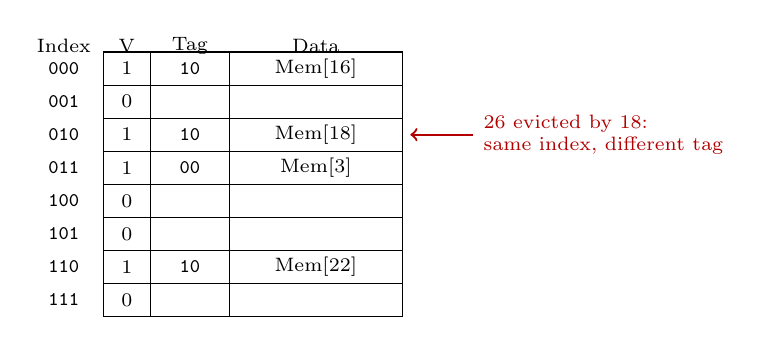
\begin{tikzpicture}[font=\scriptsize, x=1cm, y=0.42cm]
  \node at (0.4,0.7) {Index}; \node at (1.2,0.7) {V}; \node at (2.0,0.7) {Tag}; \node at (3.6,0.7) {Data};
  \foreach \i/\v/\tg/\d [count=\r from 0] in {000/1/10/{Mem[16]}, 001/0/{}/{}, 010/1/10/{Mem[18]}, 011/1/00/{Mem[3]},
      100/0/{}/{}, 101/0/{}/{}, 110/1/10/{Mem[22]}, 111/0/{}/{}} {
    \node[font=\ttfamily\scriptsize] at (0.4,-\r) {\i};
    \draw (0.9,-\r-0.5) rectangle (1.5,-\r+0.5);
    \draw (1.5,-\r-0.5) rectangle (2.5,-\r+0.5);
    \draw (2.5,-\r-0.5) rectangle (4.7,-\r+0.5);
    \node at (1.2,-\r) {\v}; \node[font=\ttfamily\scriptsize] at (2.0,-\r) {\tg}; \node at (3.6,-\r) {\d};
  }
  \draw[->, red!70!black, thick] (5.6,-2) -- (4.8,-2) node[pos=0, right, font=\scriptsize, align=left]{26 evicted by 18:\\same index, different tag};
\end{tikzpicture}
\end{center}
Hit rate $3/8$.
\end{example}

\subsection{Block size}

Larger blocks exploit spatial locality and lower the miss rate, up to a
point: with a fixed cache size, too-large blocks mean too few lines (more
conflicts), and the miss penalty grows (more data to transfer).

\section{The Three Cs of Misses}

\begin{itemize}
  \item \textbf{Compulsory} (cold): first access to a block.
  \item \textbf{Capacity}: the working set does not fit in the cache.
  \item \textbf{Conflict}: too many blocks map to the same set, even though
    the cache has room elsewhere. Reduced by associativity.
\end{itemize}

\section{Associative Caches}

\begin{itemize}
  \item \textbf{Fully associative}: a block can go in any line; compare all
    tags in parallel (expensive). No conflict misses.
  \item \textbf{$k$-way set associative}: lines grouped into sets of $k$; a
    block maps to one set ($\text{set} = \text{block address} \bmod
    \#\text{sets}$) and can occupy any of the $k$ lines there. Search $k$
    tags in parallel with $k$ comparators and a mux.
\end{itemize}
Direct-mapped is 1-way; fully associative is $N$-way. For a fixed cache
size, doubling associativity halves the number of sets: the index shrinks by
one bit and the tag grows by one bit.

\begin{figure}[H]
\centering
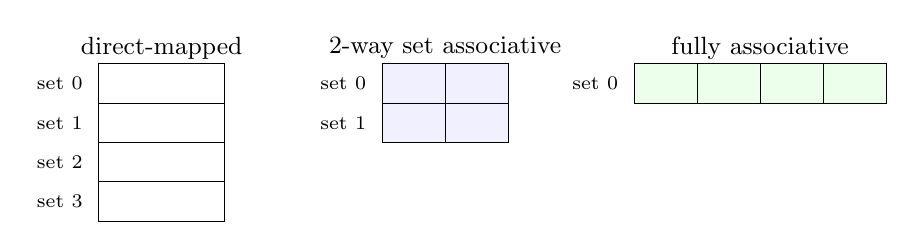
\begin{tikzpicture}[font=\scriptsize, x=0.8cm, y=0.5cm]
  % direct mapped
  \node[font=\small] at (1,1.4) {direct-mapped};
  \foreach \s in {0,...,3} {\draw (0,-\s) rectangle (2,-\s+1); \node[anchor=east] at (-0.1,-\s+0.5) {set \s};}
  % 2-way
  \node[font=\small] at (5.5,1.4) {2-way set associative};
  \foreach \s in {0,1} {\draw[fill=blue!6] (4.5,-\s) rectangle (6.5,-\s+1); \draw (5.5,-\s) -- (5.5,-\s+1);
    \node[anchor=east] at (4.4,-\s+0.5) {set \s};}
  % fully associative
  \node[font=\small] at (10.5,1.4) {fully associative};
  \draw[fill=green!8] (8.5,0) rectangle (12.5,1);
  \foreach \x in {9.5,10.5,11.5} \draw (\x,0) -- (\x,1);
  \node[anchor=east] at (8.4,0.5) {set 0};
\end{tikzpicture}
\caption{Three ways to organise the same four blocks of cache. A block
maps to one set and may occupy any way (column) of that set.}
\end{figure}

\paragraph{Replacement.} In a set-associative cache, on a miss we must pick
a victim: \textbf{LRU} (least recently used; easy for 2-way with one bit per
set), random, or FIFO.

\begin{example}
Block addresses 0, 8, 0, 6, 8 on caches with four 1-block lines.
\begin{itemize}
  \item Direct-mapped (index mod 4): 0 $\to$ 0 miss, 8 $\to$ 0 miss
    (evicts 0), 0 miss (evicts 8), 6 $\to$ 2 miss, 8 miss. 5 misses.
  \item 2-way (2 sets, LRU): 0 $\to$ set 0 miss, 8 $\to$ set 0 miss,
    0 hit, 6 $\to$ set 0 miss (evicts 8, the LRU), 8 miss (evicts 0).
    4 misses.
  \item Fully associative: 0, 8 miss, 0 hit, 6 miss, 8 hit. 3 misses.
\end{itemize}
\end{example}

\section{Writes}

\begin{itemize}
  \item \textbf{Write-through}: every write updates both cache and memory.
    Simple, memory always consistent, but slow; use a \textbf{write buffer}
    so the processor need not wait.
  \item \textbf{Write-back}: write only the cache; mark the line
    \textbf{dirty}; write it to memory when it is evicted. Less memory
    traffic but more complex.
\end{itemize}
On a write miss: \textbf{write-allocate} (fetch the block into the cache,
then write; usual with write-back) or \textbf{no-write-allocate} (write
memory only; usual with write-through).

\section{Cache Performance}

\[
\text{CPU time} = \text{IC} \times (\text{CPI}_{base} + \text{memory stall
cycles per instruction}) \times \text{cycle time},
\]
\[
\text{Stall cycles per instr.} = \frac{\text{memory accesses}}{\text{instruction}}
\times \text{miss rate} \times \text{miss penalty}.
\]

\begin{example}
Base CPI 2, I-cache miss rate 2\%, D-cache miss rate 4\%, miss penalty 100
cycles, 36\% of instructions are loads/stores.
I-stalls $= 1 \times 0.02 \times 100 = 2$;
D-stalls $= 0.36 \times 0.04 \times 100 = 1.44$.
CPI $= 2 + 2 + 1.44 = 5.44$. A perfect cache would make the machine
$5.44/2 = 2.72$ times faster.
\end{example}

\begin{example}[AMAT]
Clock 1\,ns, hit time 1 cycle, miss penalty 20 cycles, miss rate 5\%.
AMAT $= 1 + 0.05 \times 20 = 2$ cycles $= 2$\,ns.
\end{example}

\paragraph{Multilevel caches.} L1 is small and optimized for hit time; L2
(and L3) are larger and optimized for miss rate, reducing the effective miss
penalty of L1. \emph{Local} miss rate = misses / accesses to that level;
\emph{global} miss rate = misses / all CPU accesses.

\paragraph{Software.} Access patterns matter: traversing a 2D array in the
order it is stored (row-major in C) has good spatial locality; blocking
(tiling) algorithms like matrix multiply keep the working set in cache.

\section*{Summary}
\begin{itemize}
  \item Locality (temporal, spatial) makes the hierarchy work.
  \item Address = tag | index | offset; valid bit + tag comparison decides
    a hit.
  \item Direct-mapped (1 place), $k$-way set associative, fully
    associative; LRU replacement.
  \item Misses: compulsory, capacity, conflict.
  \item Write-through (+ write buffer) vs write-back (dirty bit);
    write-allocate vs no-write-allocate.
  \item AMAT = hit time + miss rate $\times$ miss penalty; stall cycles add
    to CPI.
\end{itemize}
